\documentclass[a4paper,12pt]{article}

\usepackage[utf8]{inputenc}
\usepackage[T1]{fontenc}
\usepackage[hidelinks]{hyperref}
\usepackage{commath}
\usepackage{mathtools}
\usepackage{amssymb}
\usepackage{mathrsfs}
\usepackage{libertine}
\usepackage{mortenmath}
\usepackage{graphicx}

% Make ligatures and stuff copiable from pdf:
\input{glyphtounicode}
\pdfgentounicode=1

\title{Summary of\\TTK4150 Nonlinear Control Systems}
\author{Morten Fyhn Amundsen \& Erik Liland}
\date{\today}

\begin{document}

\maketitle
\tableofcontents

\paragraph{Todo}
\begin{itemize}
	\item Estimate of $R_A$
	\item K/KL-based stability (p28 slide6)
	\item L/L-infinity stability
	\item Def. 5.1
	\item Theorem 10.4
	\item Nonvanishing perturbation.
	\item Theorem 6.3
\end{itemize}

%!TEX root = TTK4150-Summary.tex
\section{Math}

%%%%%%%%%%%%%%%%%%%%%%%%%%%%%%
\subsection{Metric norms}
%%%%%%%%%%%%%%%%%%%%%%%%%%%%%%
\paragraph{General $p$-norm}
\begin{equation}
	\norm{x}_p
	=
	\left(
		\sum_{i=1}^{n} \abs{x_i}^p
	\right)
	^{1/p}
\end{equation}

\paragraph{Taxicab norm ($p=1$)}
\begin{equation}
	\norm{x}_1
	=
	\sum_{i=1}^{n} \abs{x_i}
\end{equation}

\paragraph{Euclidean norm ($p=2$)}
\begin{equation}
	\norm{x}_2
	=
	\sqrt{x_1^2 + \cdots + x_n^2}
\end{equation}

%%%%%%%%%%%%%%%%%%%%%%%%%%%%%%
\subsection[\texorpdfstring{Boundedness and $\mathcal{L}_p$-norms}
	{Boundedness and Lp-norms}]
	{Boundedness and $\mathcal{L}_p$-norms}
%%%%%%%%%%%%%%%%%%%%%%%%%%%%%%
\paragraph{$\mathcal{L}_p$-norm}
\begin{equation}
	\norm{f}_p
	=
	\left(
		\int_a^b \abs{f(\tau)}^p \dif \tau
	\right)^{1/p}
\end{equation}

\paragraph{$\mathcal{L}_\infty$-norm}
\begin{equation}
	\norm{f}_\infty
	=
	\sup_{a \leq t \leq b} \abs{f(t)}
\end{equation}

\paragraph{Boundedness}
\begin{equation}
	f \in \mathcal{L}_p \Leftrightarrow \norm{f}_p < \infty
\end{equation}

%%%%%%%%%%%%%%%%%%%%%%%%%%%%%%
\subsection{Properties of norms}
%%%%%%%%%%%%%%%%%%%%%%%%%%%%%%
\paragraph{Hölder's inequality}
\begin{equation}
	\norm{fg}_1 \leq \norm{f}_p \norm{g}_q
\end{equation}
with $\frac{1}{p} + \frac{1}{q} = 1$.

%%%%%%%%%%%%%%%%%%%%%%%%%%%%%%
\subsection{Matrix properties}
%%%%%%%%%%%%%%%%%%%%%%%%%%%%%%
\paragraph{Singular} A matrix is \emph{singular} iff its determinant is zero.

\paragraph{Skew-symmetry} A matrix $A$ is \emph{skew-symmetric} iff
\begin{equation}
	-A = A\T
	.
\end{equation}

\paragraph{Jacobian} The \emph{Jacobian} matrix is defined by
\begin{equation}
	J
	=
	\od{f}{x}
	=
	\begin{bmatrix}
		\pd{f_1}{x_1} & \cdots & \pd{f_1}{x_n} \\
		\vdots        & \ddots & \vdots        \\
		\pd{f_m}{x_1} & \cdots & \pd{f_m}{x_n}
	\end{bmatrix}
	.
\end{equation}

\paragraph{Hurwitz}
A matrix $A$ is \emph{Hurwitz} if all eigenvalues of $A$ satisfy $\Re \lambda_i < 0$.

\paragraph{Positive definite} A matrix being \emph{positive definite} is equivalent to
\begin{itemize}
	\item all its eigenvalues being positive,
	\item all its leading principal minors being positive.
\end{itemize}
In addition, we have
\begin{equation}
	\lambda\sub{min}(H) x\T x \leq x\T H x \leq \lambda\sub{max}(H) x\T x
\end{equation}
for a positive definite $x\T H x$.
                              % Not in Khalil
%!TEX root = TTK4150-Summary.tex
\section{Seconds-order systems}
\begin{equation}\label{eq:autonomous}
	\dot{x} = f(x), \quad x \in \mathbb{R}^2
\end{equation}

%%%%%%%%%%%%%%%%%%%%%%%%%%%%%%
\subsection{Behaviour near equilibria}
%%%%%%%%%%%%%%%%%%%%%%%%%%%%%%
Linearise and find eigenvalues at each equilibrium:
\begin{itemize}
	\item Real $\lambda$
	\begin{itemize}
		\item $\lambda_1 < \lambda_2 < 0 \implies$ Stable node.
		\item $0 < \lambda_1 < \lambda_2 \implies$ Unstable node.
		\item $\lambda_1 < 0 < \lambda_2 \implies$ Saddle point.
	\end{itemize}
	\item Complex $\lambda_{1,2} = \alpha \pm \beta \imath$
	\begin{itemize}
		\item $\alpha = 0 \implies$ Center.
		\item $\alpha < 0 \implies$ Stable focus.
		\item $\alpha > 0 \implies$ Unstable focus.
	\end{itemize}
\end{itemize}

%%%%%%%%%%%%%%%%%%%%%%%%%%%%%%
\subsection{Periodic orbits}
%%%%%%%%%%%%%%%%%%%%%%%%%%%%%%
\paragraph{Lemma 2.1 (Poincaré-Bendixson criterion)}
\begin{sloppypar}
	Consider \eqref{eq:autonomous}. Let $M$ be a bounded, closed subset of the plane such that
\end{sloppypar}
\begin{itemize}
	\item $M$ contains no equilibria, or \emph{one} equilibrium for which the eigenvalues of the Jacobian has positive real parts,
	\item All trajectories in $M$ stay in $M$.
\end{itemize}
Then, $M$ contains a periodic orbit.

\paragraph{Lemma 2.2 (Bendixson (negative) criterion)}
If
\begin{equation}
	\pd{f_1}{x_1} + \pd{f_2}{x_2}
\end{equation}
is not zero and does not change sign on a simply connected region $\mathbb{D}$, then \eqref{eq:autonomous} has no periodic orbits in $\mathbb{D}$.

\paragraph{Corollary 2.1 (The index method)}
\begin{itemize}
	\item Nodes, foci, and centers have index 1.
	\item Saddle points have index -1.
\end{itemize}
The sum of indices of all equilibria within a periodic orbit is always 1.              % Chapter 2
%!TEX root = TTK4150-Summary.tex
\section{Lyapunov stability}

\paragraph{Lyapunov function (LF)}
$V(x)$ is an LF iff
\begin{itemize}
	\item $V \in C^1$
	\item $V(0) = 0$ \\
	      $V(x) > 0 \quad \forall \quad x \in \mathbb{D} \backslash \{0\}$
	\item $\dot{V}(0) = 0$ \\
	      $\dot{V}(x) \leq 0 \quad \forall \quad x \in \mathbb{D} \backslash \{0\}$
\end{itemize}

\paragraph{Strict Lyapunov function (SLF)}
$V(x)$ is an SLF iff it is an LF and
\begin{itemize}
	\item $\dot{V}(x) < 0 \quad \forall \quad x \in \mathbb{D} \backslash \{0\}$
\end{itemize}

%%%%%%%%%%%%%%%%%%%%%%%%%%%%%%
\subsection{Autonomous systems}
%%%%%%%%%%%%%%%%%%%%%%%%%%%%%%
\paragraph{Theorem 4.1 (Direct Lyapunov method)}
\begin{itemize}
	\item If $\exists$ an LF for the origin, then the origin is stable.
	\item If $\exists$ an SLF for the origin, then the origin is asymptotically stable.
\end{itemize}

\paragraph{Theorem 4.2 (GAS)}
If $\exists$ an SLF $V$ for the origin and $V$ is radially unbounded, then the origin is globally asymptotically stable.

%%%%%%%%%%%%%%%%%%%%%%%%%%%%%%
\subsection{Invariance principle}
%%%%%%%%%%%%%%%%%%%%%%%%%%%%%%
\paragraph{Invariant set} A set $M$ is an \emph{invariant set} w.r.t. $\dot{x} = f(x)$ if
\begin{equation}
	x(0) \in M \implies x(t) \in M \quad \forall t \in \mathbb{R}.
\end{equation}
(Any solution in $M$ stays in $M$ for all future and past.)

\paragraph{Theorem 4.4 (LaSalle's theorem)}
If $\exists \: V : \mathbb{D} \to \mathbb{R}$ such that
\begin{itemize}
	\item $V \in C^1$,
	\item $\exists \: c > 0$ such that $\Omega_c = \{x \in \mathbb{R}^n | V(x) \leq c \} \subseteq \mathbb{D}$ is bounded,
	\item $\dot{V}(x) \leq 0 \quad \forall \quad x \in \Omega_c$.
\end{itemize}
Let $E = \{ x \in \Omega_c | \dot{V}(x) = 0 \}$. Let $M$ be the largest invariant set in $E$. Then
\begin{equation}
	x(0) \in \Omega_c \implies x(t) \xrightarrow{t \to \infty} M.
\end{equation}

\paragraph{Corollary 4.1} Let $x^* = 0$ for $\dot{x} = f(x)$. If for an LF $V(x)$ we have $\dot{V}(x) \leq 0$ on $D$: Let $S = \{ x \in D | \dot{V}(x) = 0 \}$ and only $x(t) \equiv 0$ can stay in $S$, then $x = 0$ AS.

\paragraph{Corollary 4.2} If corollary 4.1 holds with $D = \mathbb{R}^n$, then $x = 0$ GAS.

%%%%%%%%%%%%%%%%%%%%%%%%%%%%%%
\subsection{Linear systems and linearisation}
%%%%%%%%%%%%%%%%%%%%%%%%%%%%%%
\paragraph{Theorem 4.7 (Lyapunov's indirect method)}
Let $x^* = 0$ for $\dot{x} = f(x)$ where $f : \mathbb{D} \rightarrow \mathbb{R}^n$ satisfies $f \in \mathbb{C}^1$ and $\mathbb{D}$ is a neighborhood of the origin. Let
\begin{equation}
	A = \pd{f}{x} (x) \evalat{x = 0}
\end{equation}
and $\lambda_i$ be the eigenvalues of $A$. Then
\begin{enumerate}
	\item $\Re \lambda_i < 0 \mbox{ for all } \lambda_i \implies x = 0$ AS.
	\item $\Re \lambda_i > 0 \mbox{ for any } \lambda_i \implies x = 0$ unstable.
\end{enumerate}

%%%%%%%%%%%%%%%%%%%%%%%%%%%%%%
\subsection{Comparison functions}
%%%%%%%%%%%%%%%%%%%%%%%%%%%%%%
\paragraph{Class $\mathcal{K}$ function}
A continuous function $\alpha : [0,a) \to [0, \infty)$ belongs to class $\mathcal{K}$ iff
\begin{itemize}
	\item it is stricly increasing,
	\item $\alpha(0) = 0$.
\end{itemize}

\paragraph{Class $\mathcal{K}_\infty$ function}
A continuous function $\alpha : [0,a) \to [0, \infty)$ belongs to class $\mathcal{K}_\infty$ iff
\begin{itemize}
	\item it is of class $\mathcal{K}$,
	\item $a = \infty$,
	\item $\alpha(r) \xrightarrow{r \to \infty} \infty$.
\end{itemize}

\paragraph{Class $\mathcal{KL}$ function}
A continunous function $\beta : [0,a) \times [0,\infty) \to [0,\infty)$ belongs to class $\mathcal{KL}$ if for each fixed $s$
\begin{itemize}
	\item $\beta(r,s)$ is a class $\mathcal{K}$ function w.r.t. $r$,
\end{itemize}
and for each fixed $r$
\begin{itemize}
	\item $\beta(r,s)$ is decreasing w.r.t. $s$,
	\item $\beta(r,s) \xrightarrow{s \to \infty} 0$.
\end{itemize}

%%%%%%%%%%%%%%%%%%%%%%%%%%%%%%
\subsection{Nonautonomous systems}
%%%%%%%%%%%%%%%%%%%%%%%%%%%%%%
\begin{equation}\label{eq:nonautonomous}
	\dot{x} = f(t,x), \quad f : [0,\infty) \times \mathbb{D} \to \mathbb{R}^n
\end{equation}

\paragraph{Decrescentness}
$V(t,x)$ is \emph{decrescent} iff
\begin{equation}
	\begin{rcases}
		V(t,0) =    0      \\
		V(t,x) \leq W_2(x)
	\end{rcases}
	\forall \: t \geq 0
	\mbox{, for some pos. def. }
	W_2(x).
\end{equation}

\paragraph{Theorem 4.8--4.9}
Let $V : [0,\infty) \times \mathbb{D} \to \mathbb{R}$ and $V \in C^1$ for \eqref{eq:nonautonomous}. Then $x^* = 0$ is
\begin{center}
	\begin{tabular}{lllll}
		& S & US & UAS & GUAS \\
		\hline
		$V$ & PD & PD, decr. & PD, decr. & PD, decr., RU \\
		$\dot{V}$ & NSD & NSD & ND & ND \\
		$\forall x \in$ & $\mathbb{D}$ & $\mathbb{D}$ & $\mathbb{D}$ & $\mathbb{R}^n$
	\end{tabular}
\end{center}
(PD = positive definite, decr. = decrescent, RU = radially unbounded, NSD = negative semidefinite, ND = negative definite.)

\paragraph{Theorem 4.10 (exponential stability)}
If $\exists \: a, k_1, k_2, k_3 > 0$ such that
\begin{itemize}
	\item $V \in C^1$
	\item $k_1 \norm{x}^a \leq V(x) \leq k_2 \norm{x}^a \quad \forall \: x \in \mathbb{D}$
	\item $\dot{V}(x) \leq - k_3 \norm{x}^a \quad \forall \: x \in \mathbb{D}$
\end{itemize}
then $x = 0$ ES. If $\mathbb{D} = \mathbb{R}^n$, $x = 0$ is GES.

%%%%%%%%%%%%%%%%%%%%%%%%%%%%%%
\subsection{Converse theorems}
%%%%%%%%%%%%%%%%%%%%%%%%%%%%%%
\paragraph{Corollary 4.3}
The origin of $\dot{x} = f(x)$ is ES iff $A$ is Hurwitz, where
\begin{equation}
	A =
	\begin{bmatrix}
		\pd{f}{x}
	\end{bmatrix}
	\evalat{x=0}
	.
\end{equation}

%%%%%%%%%%%%%%%%%%%%%%%%%%%%%%
\subsection{Input-to-state stability}
%%%%%%%%%%%%%%%%%%%%%%%%%%%%%%
\begin{equation}\label{eq:iss-system}
	\Sigma: \quad \dot{x} = f(t,x,u)
\end{equation}

\paragraph{Theorem 4.19}
Let $V : [0,\infty) \times \mathbb{R}^n \to \mathbb{R}$ be cont. diff.able such that
\begin{equation}
	\alpha_1 \left( ||x|| \right) \leq V(t,x) \leq \alpha_2 \left( ||x|| \right)
\end{equation}
\begin{equation}
	\dot{V} \leq -W_3(x) \quad \forall \quad ||x|| \geq \rho \left( ||u|| \right) > 0
\end{equation}
$\forall (t,x,u) \in [0,\infty) \times R^n \times R^m$, where
\begin{itemize}
	\item $\alpha_1, \alpha_2 \in \mathcal{K}_\infty$,
	\item $\rho \in \mathcal{K}$, and
	\item $W_3(x)$ is a cont. pos. def. function on $\mathbb{R}^n$.
\end{itemize}
Then, the system is ISS with $\gamma=\alpha_1^{-1} \circ \alpha_2 \circ \rho$.

\paragraph{ISS vs. 0-GUAS}
\begin{gather}
	\Sigma \mbox{ ISS} \implies \Sigma \mbox{ 0-GUAS} \\
	\neg (\Sigma \mbox{ 0-GUAS}) \implies \neg (\Sigma \mbox{ ISS})
\end{gather}

\paragraph{Lemma 4.6 (ISS vs. 0-GES)}
For \eqref{eq:iss-system} with $f \in C^1$ and $f$ globally Lipschitz in $(x,u)$, then
\begin{equation}
	\Sigma \mbox{ 0-GES} \implies \Sigma \mbox{ ISS}
	.
\end{equation}

\paragraph{Lemma 4.7}
The cascade of a GUAS and an ISS system is ISS. (Output of GUAS is the input of ISS.)
                % Chapter 4
%!TEX root = TTK4150-Summary.tex
\section{Passivity}
\begin{align}
	\dot{x} &= f(x,u) \label{eq:passive1} \\
	y       &= h(x,u) \label{eq:passive2}
\end{align}

%%%%%%%%%%%%%%%%%%%%%%%%%%%%%%
\subsection{Memoryless functions}
%%%%%%%%%%%%%%%%%%%%%%%%%%%%%%
\paragraph{Definition 6.1}
The system $y = h(t,u)$ is
\begin{itemize}
	\item passive if $u\T y \geq 0$,
	\item lossless if $u\T y = 0$,
	\item input-feedforward passive if $u\T y \geq u\T \phi(u)$ for some $\phi(u)$,
	\item input strictly passive if it is IFP and $u\T \phi(u) > 0 \: \forall \: y \neq 0$,
	\item output-feedback passive if $u\T y \geq y\T \rho(y)$ for some $\rho(y)$,
	\item output strictly passive if it is OFP and $y\T \rho(y) > 0 \: \forall \: y \neq 0$.
\end{itemize}

%%%%%%%%%%%%%%%%%%%%%%%%%%%%%%
\subsection{State models}
%%%%%%%%%%%%%%%%%%%%%%%%%%%%%%
\paragraph{Definition 6.3}
The system \eqref{eq:passive1}--\eqref{eq:passive2} with storage function $V(x) \geq 0$ is
\begin{itemize}
	\item passive if $u\T y \geq \dot{V}$,
	\item lossless if $u\T y = \dot{V}$,
	\item input-feedforward passive if $u\T y \geq \dot{V} + u\T \phi(u)$ for some function $\phi$,
	\item input strictly passive if it is IFP with $u\T \phi(u) > 0 \: \forall \: u \neq 0$,
	\item output-feedback passive if $u\T y \geq \dot{V} + y\T \rho(y)$ for some function $\rho$,
	\item output strictly passive if it is OFP with $y\T \rho(y) > 0 \: \forall \: y \neq 0$,
	\item strictly passive if $u\T y \geq \dot{V} + \psi(x)$ for some pos. def $\psi$.
\end{itemize}

%%%%%%%%%%%%%%%%%%%%%%%%%%%%%%
\subsection[\texorpdfstring{$\mathcal{L}_2$ and Lyapunov stability}
	{L2 and Lyapunov stability}]
	{$\mathcal{L}_2$ and Lyapunov stability}
%%%%%%%%%%%%%%%%%%%%%%%%%%%%%%
\paragraph{Lemma 6.5 (finite-gain $\mathcal{L}_2$ stable)}
If a system is output strictly passive with $\rho(y) = \delta y$ with $\delta > 0$ then it is finite-gain $\mathcal{L}_2$ stable with gain $\gamma \leq \delta^{-1}$.

\paragraph{Definition 6.5 (zero-state observability)}
The system \eqref{eq:passive1}--\eqref{eq:passive2} is zero-state observable if only the solution $x(t) \equiv 0$ of $\dot{x} = f(x,0)$ can stay in $S = \{ x \in \mathbb{R}^n | h(x,0) = 0 \}$.

%%%%%%%%%%%%%%%%%%%%%%%%%%%%%%
\subsection{Feedback systems}
%%%%%%%%%%%%%%%%%%%%%%%%%%%%%%
\begin{figure}[htbp]
	\centering
	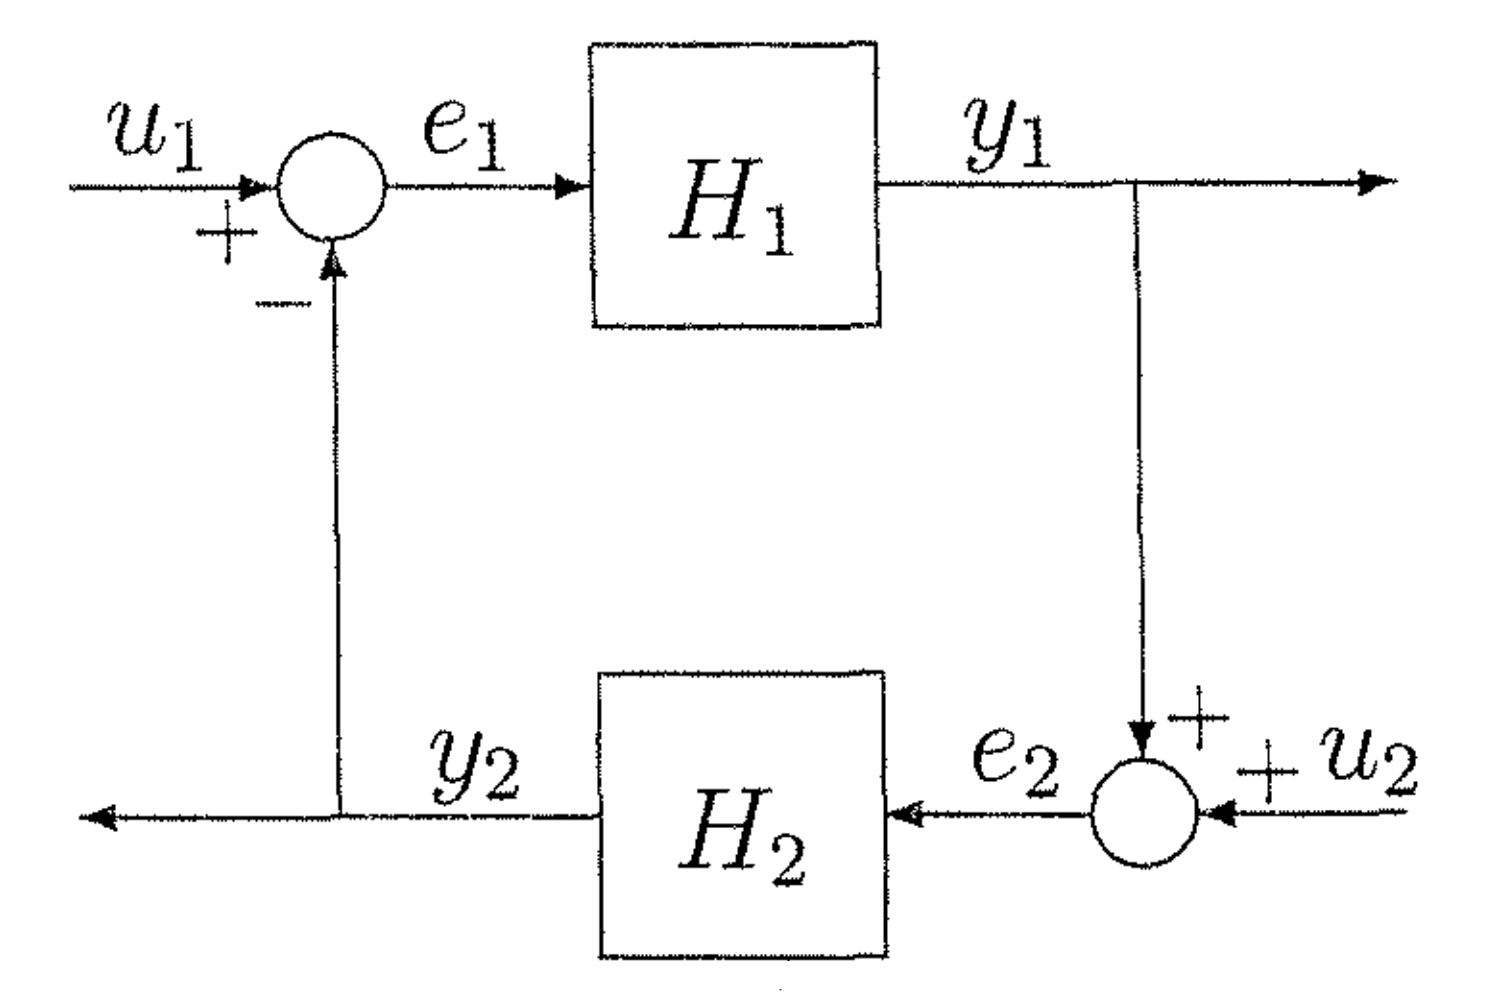
\includegraphics[width=8cm]{feedback-connection.png}
	\caption{Feedback connection}
\end{figure}

\paragraph{Theorem 6.1}
The feedback connection of two passive systems is passive, with $V = V_1 + V_2$.

\paragraph{Theorem 6.2 ($\mathcal{L}_2$-stability of feedback connection)}
If $H_1$ and $H_2$ satisfy
\begin{equation}
	e_i\T y_i \geq \dot{V}_i + \epsilon_i e_i\T e_i + \delta_i y_i\T y_i
\end{equation}
and
\begin{equation}
	\epsilon_1 + \delta_2 > 0 \mbox{ and } \epsilon_2 + \delta_1 > 0
\end{equation}
then the feedback connection is finite-gain $\mathcal{L}_2$-stable.                         % Chapter 6
%!TEX root = TTK4150-Summary.tex
\section{Stability of perturbed systems}
We consider perturbed systems on the form
\begin{equation}
	\dot{x} = f(t,x) + g(t,x)
\end{equation}
with \emph{nominal} systems
\begin{equation}
	\dot{x} = f(t,x)
	.
\end{equation}

%%%%%%%%%%%%%%%%%%%%%%%%%%%%%%
\subsection{Vanishing perturbation}
%%%%%%%%%%%%%%%%%%%%%%%%%%%%%%
\paragraph{Lemma 9.1}
\begin{itemize}
	\item The origin is an ES equilibrium of the nominal system.
	\item $V(t,x)$ is an LF of the nominal system, and satisfies
		\begin{equation}
			c_1 \norm{x}^2 \leq V(t,x) \leq c_2 \norm{x}^2
		\end{equation}
		and
		\begin{equation}
			\norm{\pd{V}{x}} \leq c_4 \norm{x}
			.
		\end{equation}
	\item The perturbation $g(t,x)$ satisfies
		\begin{equation}
			\norm{g(t,x)} \leq \gamma \norm{x}, \quad \gamma < \frac{c_3}{c_4}
			.
		\end{equation}
\end{itemize}
Then $x^* = 0$ of the perturbed system is ES. If the assumptions hold globally, $x = 0$ is GES.


%%%%%%%%%%%%%%%%%%%%%%%%%%%%%%
\subsection{Nonvanishing perturbation}
%%%%%%%%%%%%%%%%%%%%%%%%%%%%%%    % Chapter 9
%!TEX root = TTK4150-Summary.tex
\section{Perturbation theory and averaging}
\begin{equation}\label{eq:perturbed}
	\dot{x} = f(x) + \epsilon g(t,x,\epsilon)
\end{equation}

%%%%%%%%%%%%%%%%%%%%%%%%%%%%%%
\subsection{Periodic perturbation of autonomous systems}
%%%%%%%%%%%%%%%%%%%%%%%%%%%%%%
\paragraph{Definition of $P_\epsilon(x)$:}
$\phi(t;t_0,x_0,\epsilon)$ is the solution of \eqref{eq:perturbed} that starts at $(t_0,x_0)$. $P_\epsilon(x)$ is
\begin{equation}
	P_\epsilon(x) = \phi(T;0,x,\epsilon)
\end{equation}

\paragraph{Lemma 10.1}
The system \eqref{eq:perturbed} has a T-periodic solution iff
\begin{equation}
	x = P_\epsilon(x)
\end{equation}
has a solution.

%%%%%%%%%%%%%%%%%%%%%%%%%%%%%%
\subsection{Averaging}
%%%%%%%%%%%%%%%%%%%%%%%%%%%%%%
 % Chapter 10
%!TEX root = TTK4150-Summary.tex
\section{Feedback linearization}
Consider a class of nonlinear systems of the form

\begin{equation}\label{eq:nonlinear-system}
	\begin{split}
		\dot{x} &= f(x) + G(x)u             \\
		y       &= h(x)                     \\
		u       &= \alpha (x) + \beta (x) v \\
		z       &= T(x)
	\end{split}
\end{equation}
where $u$ is a state feedback conboller, and $T$ is a change of variables.

To be able to cancel nonlinearities with feedback the input and non-linearities must appear together as a sum $\lambda (x) + u$ or as a product $\lambda (x) u$, where the matrix $\lambda(x)$ is non-singular in the domain of interest, and $u = \beta(x) v, \beta(x) = \lambda^{-1}$.

\paragraph{Definition 13.1}
A nonlinear system as \eqref{eq:nonlinear-system} where $f:D \to R^n$ and $G : D \to R^{n \times p}$ are sufficiently smooth on a domain $D \subseteq R^n$, is said to be feedback linearizable  (or input-state linearizable) if there exists a diffeomorphism $T:D \to R^n$ such that $D_z = T(D)$ contains the origin and the change of variables $z = T(x)$ transforms \eqref{eq:nonlinear-system} into the form
\begin{equation}
	\dot{z} = Az + B\lambda (x) [u - \alpha(x)]
\end{equation}
with $(A,B)$ controllable and $\lambda(x)$ nonsingular $\forall x \in D$.

%%%%%%%%%%%%%%%%%%%%%%%%%%%%%%
\subsection{Input-output linearization}
%%%%%%%%%%%%%%%%%%%%%%%%%%%%%%
Consider \eqref{eq:nonlinear-system} which satisfies Def. 13.1. The derivative $\dot{y}$ is given by
\begin{equation}
	\dot{y} = \pd{h}{x} \del{f(x) + g(x)} \triangleq L_f h(x) + L_g h(x) u
\end{equation}
where $L_f h(x) \triangleq \pd{h}{x} f(x) $ is the \emph{Lie Derivative} of $h$ w.r.t. $f$.

\paragraph{Relative degree}
The relative degree is the number of times $y$ must be differentiated until $u \in D_0 \subseteq D$ appears. A system must have a well defined relative degree to be input-output linearizable. (It must also be minimum phase.)

\paragraph{Diffeomorphism}
Wikipedia: \emph{In mathematics, a diffeomorphism is an isomorphism of smooth manifolds. It is an invertible function that maps one differentiable manifold to another such that both the function and its inverse are smooth.}

\paragraph{Theorem 13.1}
Consider \eqref{eq:nonlinear-system} with relative degree $\rho \leq n$ in D. If $\rho = n$, then for every $x_0 \in D$, a neighborhood N of $x_0$ exists such that the map
\begin{equation}
	T(x) =
	\left[
	\begin{array}{ccc}
		h(x)     \\
		L_f h(x) \\
		\vdots   \\
		L_f^{n-1} h(x)
	\end{array}
	\right]
\end{equation}
restricted to N, is a diffeomorphism on N. If $\rho < n$, then, for every $x_0 \in D$, a neighborhood N of $x_0$ and smooth function $\phi_1 (x), \dots , \phi_{n-\rho} (x)$ exist such that 
\begin{equation}
	\pd{\phi_i}{x} g(x) = 0, \mbox{ for } 1 \leq i \leq n-\rho, \forall x \in D_0
\end{equation}
is satisfied $\forall x \in N$ and the map
\begin{equation}
	z = T(x) =
	\left[
	\begin{array}{ccc}
		\phi_1(x)         \\
		\vdots            \\
		\phi_{n-\rho}(x)  \\
		---               \\
		h(x)              \\
		\vdots            \\
		L_f^{\rho-1} h(x)
	\end{array}
	\right]
	\triangleq
	\left[
	\begin{array}{ccc}
		\phi(x) \\
		---     \\
		\psi(x)
	\end{array}
	\right]
	\triangleq
	\left[
	\begin{array}{ccc}
		\eta \\
		---  \\
		\xi
	\end{array}
	\right]
\end{equation}
restricted to N, is a diffeomorphism on N.

\paragraph{Method}
\begin{enumerate}
	\item Set system on following form $\dot{x} = f(x) + g(x)u$
	\item Find the relative degree $\rho$, ($\rho = n \Rightarrow$ no internal dynamics)
	\item Write the system in normal form (external and internal dynamics)
	\item Choose $u$ to cancel the nonlinearities
	\item Analyze the zero-dynamics
	\item Choose $v$ to solve the control problem
\end{enumerate}

%%%%%%%%%%%%%%%%%%%%%%%%%%%%%%
\subsection{Full-state linearization}
%%%%%%%%%%%%%%%%%%%%%%%%%%%%%%

%%%%%%%%%%%%%%%%%%%%%%%%%%%%%%
\subsection{State feedback control}
%%%%%%%%%%%%%%%%%%%%%%%%%%%%%%
            % Chapter 13
% %!TEX root = TTK4150-Summary.tex
\section{Feedback linearisation}

%%%%%%%%%%%%%%%%%%%%%%%%%%%%%%
\subsection{Input-output linearisation}
%%%%%%%%%%%%%%%%%%%%%%%%%%%%%%
\begin{align}
	\dot{x} &= f(x) + g(x)u \label{eq:siso-x} \\
	y       &= h(x)         \label{eq:siso-y}
\end{align}

\paragraph{Definition 13.2 (relative degree)}
The relative degree $\rho$ of \eqref{eq:siso-x}--\eqref{eq:siso-y} is equal to the number of times $y$ must be differentiated until $u$ appears.

\paragraph{Theorem 13.1}
The system \eqref{eq:siso-x} can be input-output linearised if the relative degree is well defined in the region of interest $\mathbb{D}_0$.

\paragraph{Minimum phase}
The system \eqref{eq:siso-x}--\eqref{eq:siso-y} is \emph{minimum phase} if, for the zero-dynamics $\dot{\eta} = f_0(\eta,0)$, $\eta = 0$ is AS.

\paragraph{Method}
The system is given by \eqref{eq:siso-x}--\eqref{eq:siso-y}. First determine relative degree $\rho$. Define
\begin{equation}
	\xi =
	\begin{bmatrix}
		\xi_1 \\ \vdots \\ \xi_\rho
	\end{bmatrix}
	=
	\begin{bmatrix}
		y \\ \vdots \\ y^{(\rho-1)}
	\end{bmatrix}
\end{equation}
so that
\begin{equation}
	\dot{\xi} =
	\begin{bmatrix}
		\dot{\xi}_1 \\ \vdots \\ \dot{\xi}_\rho
	\end{bmatrix}
	=
	\begin{bmatrix}
		\xi_2 \\ \vdots \\ L_f^\rho h + L_g L_f^{\rho-1} h \cdot u
	\end{bmatrix}
	.
\end{equation}
Then choose $n-\rho$ coordinates
\begin{equation}
	\eta =
	\begin{bmatrix}
		\eta_1 \\ \vdots \\ \eta_{n-\rho}
	\end{bmatrix}
\end{equation}
with the coordinate transformation
\begin{equation}
	z = T(x) =
	\begin{bmatrix}
		\eta_1 \\ \vdots \\ \eta_{n-\rho} \\ \xi_1 \\ \vdots \\ \xi_\rho
	\end{bmatrix}
\end{equation}
and choose $\eta$ such that
\begin{itemize}
	\item $T$ is a diffeomorphism,
	\item $L_g \eta_i = 0$,
	\item $\eta_i(0) = 0$.
\end{itemize}
We have then that
\begin{equation}
	\dot{\eta}_j = \pd{\eta_j}{x} \dot{x} = L_f \eta_j + \underbrace{L_g \eta_j}_{= 0} \cdot u = f_{0_j} (\eta_i, \xi_i)
\end{equation}
and we can write the system on normal form
\begin{equation}
	\begin{bmatrix}
		\dot{\eta}_1        \\
		\vdots              \\
		\dot{\eta}_{n-\rho} \\
		\dot{\xi}_1         \\
		\vdots              \\
		\dot{\xi}_\rho
	\end{bmatrix}
	=
	\begin{bmatrix}
		f_{0_1}(\eta_i, \xi_i)        \\
		\vdots                        \\
		f_{0_{n-\rho}}(\eta_i, \xi_i) \\
		\xi_2                         \\
		\vdots                        \\
		L_f^\rho h + L_g L_f^{\rho-1} h \cdot u
	\end{bmatrix}
	.
\end{equation}
Then choose $u$ to cancel the nonlinearities:
\begin{equation}
	u = \frac{1}{L_g L_f^{\rho-1} h} (-L_f^\rho h + v)
\end{equation}
This leads to
\begin{gather}
	\dot{\eta} = f_0(\eta,\xi) \\
	\dot{\xi} = 
	\begin{bmatrix}
		\xi_2 \\ \vdots \\ v
	\end{bmatrix}
\end{gather}
Then analyse the zero-dynamics---the internal dynamics when the output is kept zero by the input:
\begin{equation}
	\dot{\eta} = f_0(\eta,0)
\end{equation}                      % Also chapter 13
%!TEX root = TTK4150-Summary.tex
\section{Nonlinear design tools}

%%%%%%%%%%%%%%%%%%%%%%%%%%%%%%
\subsection{Backstepping}
%%%%%%%%%%%%%%%%%%%%%%%%%%%%%%
\paragraph{General idea}
Start by selecting a state $x_i$, where $i$ is some index. Given $\dot{x}_i = f_i(x)$, consider one of the other states present in $f_i$ as the input. Let's call this state $x_j$. Find an expression $x_j = \phi_j(x)$ that stabilizes $x_i$. (Using a Lyapunov function $V(x_i)$.) Then, define $z_j = x_j - \phi_j(x)$, and rewrite the system in terms of $x_i$ and $z_j$. Now, considering $\dot{z}_j$, use the same method to find an expression for a state present in $\dot{z}_j$ to stabilize $z_j$ and $x_i$. (Now with a Lyapunov function $V(x_i, z_j)$.) Keep going until you run out of states to stabilize.

%%%%%%%%%%%%%%%%%%%%%%%%%%%%%%
\subsection{Passivity-based control}
%%%%%%%%%%%%%%%%%%%%%%%%%%%%%%
\begin{align}
	\dot{x} &= f(x,u) \label{eq:pin-pout-x} \\
	y       &= h(x)   \label{eq:pin-pout-y}
\end{align}

\paragraph{Theorem 14.4}
If \eqref{eq:pin-pout-x}--\eqref{eq:pin-pout-y} is
\begin{itemize}
	\item passive with an RU, pos. def. storage function,
	\item zero-state observable
\end{itemize}
then $x = 0$ can be globally stabilized by $u = -\phi(y)$, with $\phi$ locally Lipschitz with $\phi(0) = 0$, $y\T \phi(y) > 0 \forall y \neq 0$.
            % Chapter 14

\end{document}
